\documentclass[11pt,a4paper]{report}
\usepackage[textwidth=37em,vmargin=30mm]{geometry}
\usepackage{calc,xunicode,amsmath,amssymb,paralist,enumitem,tabu,booktabs,datetime2,xeCJK,xeCJKfntef,listings}
\usepackage{tocloft,fancyhdr,tcolorbox,xcolor,graphicx,eso-pic,xltxtra,xelatexemoji}

\newcommand{\envyear}[0]{2025}
\newcommand{\envdatestr}[0]{2025-06-14}
\newcommand{\envfinaldir}[0]{webdb/2025/20250614/final}

\usepackage[hidelinks]{hyperref}
\hypersetup{
    colorlinks=false,
    pdfpagemode=FullScreen,
    pdftitle={Web Digest - \envdatestr}
}

\setlength{\cftbeforechapskip}{10pt}
\renewcommand{\cftchapfont}{\rmfamily\bfseries\large\raggedright}
\setlength{\cftbeforesecskip}{2pt}
\renewcommand{\cftsecfont}{\sffamily\small\raggedright}

\setdefaultleftmargin{2em}{2em}{1em}{1em}{1em}{1em}

\usepackage{xeCJK,xeCJKfntef}
\xeCJKsetup{PunctStyle=plain,RubberPunctSkip=false,CJKglue=\strut\hskip 0pt plus 0.1em minus 0.05em,CJKecglue=\strut\hskip 0.22em plus 0.2em}
\XeTeXlinebreaklocale "zh"
\XeTeXlinebreakskip = 0pt


\setmainfont{Brygada 1918}
\setromanfont{Brygada 1918}
\setsansfont{IBM Plex Sans}
\setmonofont{JetBrains Mono NL}
\setCJKmainfont{Noto Serif CJK SC}
\setCJKromanfont{Noto Serif CJK SC}
\setCJKsansfont{Noto Sans CJK SC}
\setCJKmonofont{Noto Sans CJK SC}

\setlength{\parindent}{0pt}
\setlength{\parskip}{8pt}
\linespread{1.15}

\lstset{
	basicstyle=\ttfamily\footnotesize,
	numbersep=5pt,
	backgroundcolor=\color{black!5},
	showspaces=false,
	showstringspaces=false,
	showtabs=false,
	tabsize=2,
	captionpos=b,
	breaklines=true,
	breakatwhitespace=true,
	breakautoindent=true,
	linewidth=\textwidth
}






\newcommand{\coverpic}[2]{
    % argv: itemurl, authorname
    Cover photo by #2~~(\href{#1}{#1})
}
\newcommand{\makeheader}[0]{
    \begin{titlepage}
        % \newgeometry{hmargin=15mm,tmargin=21mm,bmargin=12mm}
        \begin{center}
            
            \rmfamily\scshape
            \fontspec{BaskervilleF}
            \fontspec{Old Standard}
            \fontsize{59pt}{70pt}\selectfont
            WEB\hfill DIGEST
            
            \vfill
            % \vskip 30pt
            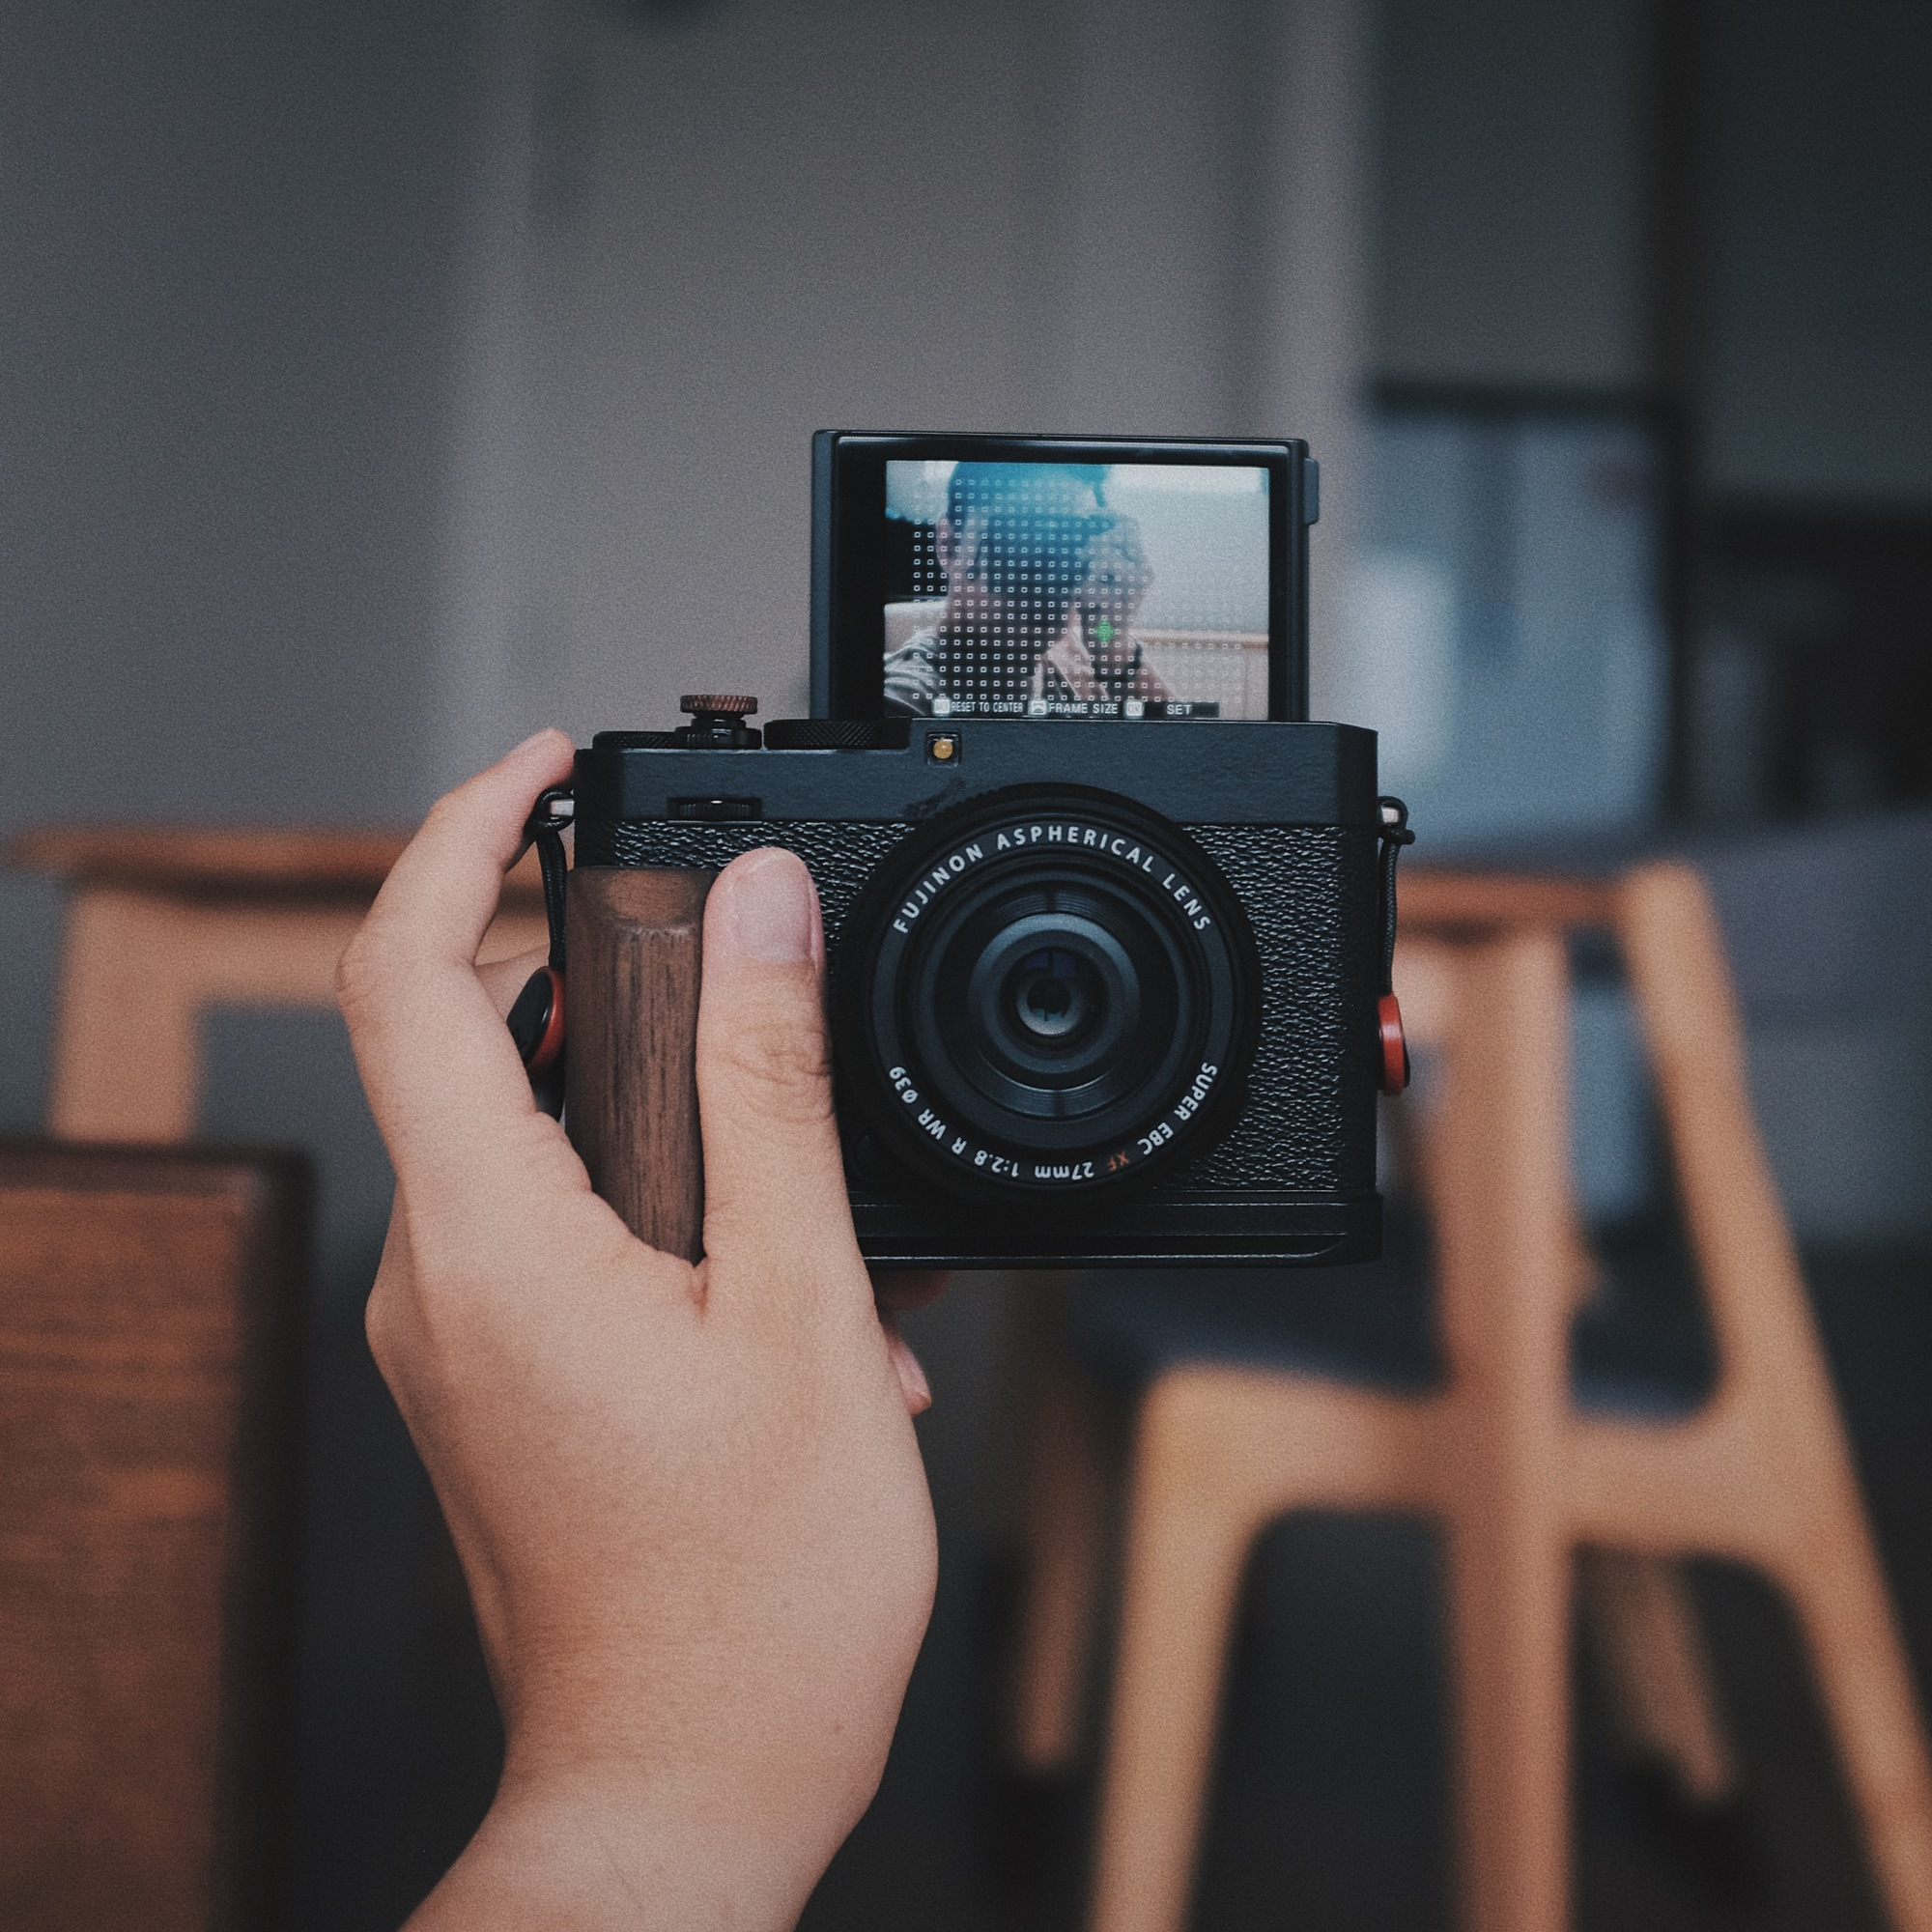
\includegraphics[width=\linewidth]{\envfinaldir/coverpic-prod.jpg}\par
            % \vskip 30pt
            \vfill

            \normalsize\rmfamily\scshape
            \copyright{} The Web Digest Project \hfill\large \envdatestr
        \end{center}
    \end{titlepage}
    % \restoregeometry
}
\newcommand{\simplehref}[1]{%
    \textcolor{blue!80!green}{\href{#1}{#1}}%
}
\renewcommand{\contentsname}{\center\Huge\sffamily\bfseries Contents\par\vskip 20pt}
\newcounter{ipartcounter}
\setcounter{ipartcounter}{0}
\newcommand{\ipart}[1]{
    % \vskip 20pt
    \clearpage
    \stepcounter{ipartcounter}
    \phantomsection
    \addcontentsline{toc}{chapter}{#1}
    % \begin{center}
    %     \Huge
    %     \sffamily\bfseries
    %     #1
    % \end{center}
    % \vskip 20pt plus 7pt
}
\newcounter{ichaptercounter}
\setcounter{ichaptercounter}{0}
\newcommand{\ichapter}[1]{
    % \vskip 20pt
    \clearpage
    \stepcounter{ichaptercounter}
    \phantomsection
    \addcontentsline{toc}{section}{\numberline{\arabic{ichaptercounter}}#1}
    \begin{center}
        \Huge
        \sffamily\bfseries
        #1
    \end{center}
    \vskip 20pt plus 7pt
}
\newcommand{\entrytitlefont}[1]{\subsection*{\raggedright\Large\sffamily\bfseries#1}}
\newcommand{\entryitemGeneric}[2]{
    % argv: title, url
    \parbox{\linewidth}{
        \entrytitlefont{#1}\par\vskip 5pt
        \footnotesize\ttfamily\mdseries
        \simplehref{#2}
    }\vskip 11pt plus 11pt minus 1pt
}
\newcommand{\entryitemGithub}[3]{
    % argv: title, url, desc
    \parbox{\linewidth}{
        \entrytitlefont{#1}\par\vskip 5pt
        \footnotesize\ttfamily\mdseries
        \simplehref{#2}\par\vskip 5pt
        \small\rmfamily\mdseries#3
    }\vskip 11pt plus 11pt minus 1pt
}
\newcommand{\entryitemAp}[3]{
    % argv: title, url, desc
    \parbox{\linewidth}{
        \entrytitlefont{#1}\par\vskip 5pt
        \footnotesize\ttfamily\mdseries
        \simplehref{#2}\par\vskip 5pt
        \small\rmfamily\mdseries#3
    }\vskip 11pt plus 11pt minus 1pt
}
\newcommand{\entryitemHackernews}[3]{
    % argv: title, hnurl, rawurl
    % \parbox{\linewidth}{
    %     \entrytitlefont{#1}\par\vskip 5pt
    %     \footnotesize\ttfamily\mdseries
    %     \simplehref{#3}\par
    %     \textcolor{black!50}{\href{#2}{#2}}
    % }\vskip 11pt plus 11pt minus 1pt
    \begin{minipage}{\linewidth}
            \entrytitlefont{#1}\par\vskip 5pt
            \footnotesize\ttfamily\mdseries
            \simplehref{#3}\par
            \textcolor{black!50}{\href{#2}{#2}}
    \end{minipage}\par\vskip 11pt plus 11pt minus 1pt
}







\begin{document}

\makeheader

\tableofcontents\clearpage




\ipart{Developers}
\ichapter{Hacker News}
\entryitemTwoLinks{Apple's Liquid Glass is prep work for AR interfaces, not just a design refresh}{https://news.ycombinator.com/item?id=44271630}{https://omc345.substack.com/p/from-skeuomorphic-to-liquid-glass}

\entryitemTwoLinks{I convinced HP's board to buy Palm and watched them kill it}{https://news.ycombinator.com/item?id=44270709}{https://philmckinney.substack.com/p/i-convinced-hps-board-to-buy-palm}

\entryitemTwoLinks{Luxe Game Engine}{https://news.ycombinator.com/item?id=44269270}{https://luxeengine.com/}

\entryitemTwoLinks{Ask HN: Is ageism in tech still a problem?}{https://news.ycombinator.com/item?id=44269225}{https://news.ycombinator.com/item?id=44269225}

\entryitemTwoLinks{OxCaml - a set of extensions to the OCaml programming language.}{https://news.ycombinator.com/item?id=44268782}{https://oxcaml.org/}

\entryitemTwoLinks{Show HN: Tattoy – a text-based terminal compositor}{https://news.ycombinator.com/item?id=44268644}{https://tattoy.sh}

\entryitemTwoLinks{Ask HN: How do I give back to people helped me when I was young and had nothing?}{https://news.ycombinator.com/item?id=44268448}{https://news.ycombinator.com/item?id=44268448}

\entryitemTwoLinks{Meta invests \$14.3B in Scale AI to kick-start superintelligence lab}{https://news.ycombinator.com/item?id=44268197}{https://www.nytimes.com/2025/06/12/technology/meta-scale-ai.html}

\entryitemTwoLinks{Anker is recalling over 1.1M power banks due to fire and burn risks}{https://news.ycombinator.com/item?id=44267989}{https://www.theverge.com/news/686084/anker-recall-uscpsc-power-bank-battery-powercore-a1263}

\entryitemTwoLinks{The European public DNS that makes your Internet safer}{https://news.ycombinator.com/item?id=44267091}{https://www.dns0.eu}

\entryitemTwoLinks{If the moon were only 1 pixel: A tediously accurate solar system model (2014)}{https://news.ycombinator.com/item?id=44266828}{https://joshworth.com/dev/pixelspace/pixelspace\_solarsystem.html}

\entryitemTwoLinks{Show HN: I wrote a BitTorrent Client from scratch}{https://news.ycombinator.com/item?id=44265851}{https://github.com/piyushgupta53/go-torrent-client}

\entryitemTwoLinks{Rendering Crispy Text on the GPU}{https://news.ycombinator.com/item?id=44265233}{https://osor.io/text}

\entryitemTwoLinks{Jemalloc Postmortem}{https://news.ycombinator.com/item?id=44264958}{https://jasone.github.io/2025/06/12/jemalloc-postmortem/}

\entryitemTwoLinks{Israel launches strikes against Iran, Defense Minister says}{https://news.ycombinator.com/item?id=44264586}{https://www.cnn.com/2025/06/12/middleeast/israel-iran-strikes-intl-hnk}

\entryitemTwoLinks{Major sugar substitute found to impair brain blood vessel cell function}{https://news.ycombinator.com/item?id=44264494}{https://medicalxpress.com/news/2025-06-major-sugar-substitute-impair-brain.html}

\entryitemTwoLinks{The Case for Software Craftsmanship in the Era of Vibes}{https://news.ycombinator.com/item?id=44264376}{https://zed.dev/blog/software-craftsmanship-in-the-era-of-vibes}

\entryitemTwoLinks{A dark adtech empire fed by fake CAPTCHAs}{https://news.ycombinator.com/item?id=44263780}{https://krebsonsecurity.com/2025/06/inside-a-dark-adtech-empire-fed-by-fake-captchas/}

\entryitemTwoLinks{Sen. Padilla is forcefully removed from Noem's news conference and handcuffed}{https://news.ycombinator.com/item?id=44263140}{https://apnews.com/article/alex-padilla-noem-immigration-protest-california-f67d220a0254473c53c16aa96f554239}

\entryitemTwoLinks{Worldwide power grid with glass insulated HVDC cables}{https://news.ycombinator.com/item?id=44262537}{https://omattos.com/2025/06/12/glass-hvdc-cables.html}\ichapter{Dribbble}
\entryitemGeneric{\hskip 0pt{}Aquasan}{https://dribbble.com/shots/26100535-Aquasan}

\entryitemGeneric{\hskip 0pt{}Eagle}{https://dribbble.com/shots/26099428-Eagle}

\entryitemGeneric{\hskip 0pt{}Mnp Technologies - Logo Design}{https://dribbble.com/shots/26092034-Mnp-Technologies-Logo-Design}

\entryitemGeneric{\hskip 0pt{}Singular Logo Concept (Unused)}{https://dribbble.com/shots/26091755-Singular-Logo-Concept-Unused}

\entryitemGeneric{\hskip 0pt{}Cre8tera // Website}{https://dribbble.com/shots/26091009-Cre8tera-Website}

\entryitemGeneric{\hskip 0pt{}Cool Pool Logo Design - Letter C Monogram}{https://dribbble.com/shots/26091401-Cool-Pool-Logo-Design-Letter-C-Monogram}

\entryitemGeneric{\hskip 0pt{}Gorilla + Bar Chart Logo}{https://dribbble.com/shots/26092670-Gorilla-Bar-Chart-Logo}

\entryitemGeneric{\hskip 0pt{}zeero logo design}{https://dribbble.com/shots/26087342-zeero-logo-design}

\entryitemGeneric{\hskip 0pt{}Create email inbox composition}{https://dribbble.com/shots/26083118-Create-email-inbox-composition}

\entryitemGeneric{\hskip 0pt{}Shori Brand}{https://dribbble.com/shots/26088139-Shori-Brand}

\entryitemGeneric{\hskip 0pt{}Roaring Bear}{https://dribbble.com/shots/26087788-Roaring-Bear}

\entryitemGeneric{\hskip 0pt{}Eagle}{https://dribbble.com/shots/26085536-Eagle}

\entryitemGeneric{\hskip 0pt{}Hand-drawn illustration pack}{https://dribbble.com/shots/26084735-Hand-drawn-illustration-pack}

\entryitemGeneric{\hskip 0pt{}Dog Mascot Various Poses}{https://dribbble.com/shots/26087977-Dog-Mascot-Various-Poses}

\entryitemGeneric{\hskip 0pt{}Branding Concept for Europe}{https://dribbble.com/shots/26087652-Branding-Concept-for-Europe}

\entryitemGeneric{\hskip 0pt{}B2B Dashboard \& Web App UI UX Design for Carbon Solutions}{https://dribbble.com/shots/26076624-B2B-Dashboard-Web-App-UI-UX-Design-for-Carbon-Solutions}

\entryitemGeneric{\hskip 0pt{}Patriot Logo Design (Unused for Sale)}{https://dribbble.com/shots/26081047-Patriot-Logo-Design-Unused-for-Sale}

\entryitemGeneric{\hskip 0pt{}Heliopoint}{https://dribbble.com/shots/26081987-Heliopoint}

\entryitemGeneric{\hskip 0pt{}Apple}{https://dribbble.com/shots/26084067-Apple}

\entryitemGeneric{\hskip 0pt{}Illustration}{https://dribbble.com/shots/26083223-Illustration}

\entryitemGeneric{\hskip 0pt{}Europe Logo Animation}{https://dribbble.com/shots/26082596-Europe-Logo-Animation}

\entryitemGeneric{\hskip 0pt{}Arc Logo}{https://dribbble.com/shots/26083648-Arc-Logo}

\entryitemGeneric{\hskip 0pt{}Heyo Turns 2!}{https://dribbble.com/shots/26078572-Heyo-Turns-2}

\entryitemGeneric{\hskip 0pt{}Fox Brand Mascot}{https://dribbble.com/shots/26077954-Fox-Brand-Mascot}


\ipart{Developers~~~~(zh-Hans)}
\ichapter{Solidot}
\entryitemGeneric{\hskip 0pt{}丹麦一政府部门准备淘汰 Windows 和 Microsoft 365}{https://www.solidot.org/story?sid=81552}

\entryitemGeneric{\hskip 0pt{}研究认为霸王龙的大型化始于亚洲}{https://www.solidot.org/story?sid=81551}

\entryitemGeneric{\hskip 0pt{}两名欧洲记者的手机感染了以色列间谍软件 Paragon}{https://www.solidot.org/story?sid=81550}

\entryitemGeneric{\hskip 0pt{}Scale AI 亚历山大·王的创业法则:人类计算资源可像计算机一样编排,吴恩达一观点毁掉红杉投资,YC创始人一句话带来商业灵感}{https://www.solidot.org/story?sid=81549}

\entryitemGeneric{\hskip 0pt{}Anker 召回逾百万台有起火风险的移动电源}{https://www.solidot.org/story?sid=81545}

\entryitemGeneric{\hskip 0pt{}马斯克威胁起诉广告商取得部分成效}{https://www.solidot.org/story?sid=81544}

\entryitemGeneric{\hskip 0pt{}四天工作制能提高生产力}{https://www.solidot.org/story?sid=81543}

\entryitemGeneric{\hskip 0pt{}谷歌CEO皮查伊两小时访谈:AI是人类所见过最深远的技术,意义将超越火与电,因为它可以自我迭代}{https://www.solidot.org/story?sid=81542}

\entryitemGeneric{\hskip 0pt{}印度航空发生致命空难,至少 200 人死亡}{https://www.solidot.org/story?sid=81541}

\entryitemGeneric{\hskip 0pt{}迪士尼和 NBC 起诉 Midjourney 侵犯版权}{https://www.solidot.org/story?sid=81540}

\entryitemGeneric{\hskip 0pt{}韦伯观测到下沙雨的气态巨行星}{https://www.solidot.org/story?sid=81539}

\entryitemGeneric{\hskip 0pt{}MS Office 的版本控制从 Source Depot 迁移到 Git}{https://www.solidot.org/story?sid=81538}

\entryitemGeneric{\hskip 0pt{}1997年,乔布斯在WWDC闭幕环节做了唯一一场即兴问答:我们要做``更好的产品'',而非``不同的产品'',十年后,iPhone发布}{https://www.solidot.org/story?sid=81537}

\entryitemGeneric{\hskip 0pt{}印度宇航员将搭乘 Axiom Space 的飞船前往国际空间站}{https://www.solidot.org/story?sid=81536}

\entryitemGeneric{\hskip 0pt{}太阳活动与 Starlink 卫星大量坠落相关}{https://www.solidot.org/story?sid=81535}

\entryitemGeneric{\hskip 0pt{}新闻网站来自 Google 的流量大幅下降}{https://www.solidot.org/story?sid=81534}

\entryitemGeneric{\hskip 0pt{}如果将所有人类都塞进肉球}{https://www.solidot.org/story?sid=81533}

\entryitemGeneric{\hskip 0pt{}因编辑反对维基百科叫停了 AI 生成文章摘要的实验}{https://www.solidot.org/story?sid=81529}

\entryitemGeneric{\hskip 0pt{}研究人员发现两个能完全绕过 Secure Boot 的漏洞利用,微软只给一个打上补丁}{https://www.solidot.org/story?sid=81528}

\entryitemGeneric{\hskip 0pt{}韦伯拍摄到寒冷气态巨行星的直接影像}{https://www.solidot.org/story?sid=81527}\ichapter{V2EX}
\entryitemGeneric{\hskip 0pt{}[推广] 🔥「游戏首免」👍一款得过奖的独立开发者游戏巨作应用,不容错过。}{https://www.v2ex.com/t/1138517}

\entryitemGeneric{\hskip 0pt{}[游戏开发] Unity 有没有什么插件可以自动把身体 Mesh 的 Weight 同步到服装 Mesh 上?分开建模大幅度动作紧身衣会露出一些小洞/接缝有好的解决方案么,尝试过 AI 提的用 Mesh Baker 合并两个 Mesh 方案,没效果}{https://www.v2ex.com/t/1138515}

\entryitemGeneric{\hskip 0pt{}[Apple TV] Quantumult X Apple TV 版要怎么查看节点延迟}{https://www.v2ex.com/t/1138514}

\entryitemGeneric{\hskip 0pt{}[宽带症候群] 广移已经无法正常使用 HK 区域节点了}{https://www.v2ex.com/t/1138513}

\entryitemGeneric{\hskip 0pt{}[汽车] [求助]只有车辆的终身使用权,要不要买?}{https://www.v2ex.com/t/1138512}

\entryitemGeneric{\hskip 0pt{}[路由器] 有玩手搓 CPE 的大佬(WH3000 PRO)}{https://www.v2ex.com/t/1138511}

\entryitemGeneric{\hskip 0pt{}[宽带症候群] 福州电信商宽也开始 qos 了吗}{https://www.v2ex.com/t/1138510}

\entryitemGeneric{\hskip 0pt{}[分享创造] 一个简单的 Icon 色彩转换器}{https://www.v2ex.com/t/1138509}

\entryitemGeneric{\hskip 0pt{}[新手求助] 新人来报道!想问问大家在哪里可以发需求}{https://www.v2ex.com/t/1138508}

\entryitemGeneric{\hskip 0pt{}[问与答] 虽然选择很多但是主流还是在用一些常见软件}{https://www.v2ex.com/t/1138507}

\entryitemGeneric{\hskip 0pt{}[分享创造] 写了个追番小工具《日本动漫人气榜》,来看看你的 30 年追番记录吧}{https://www.v2ex.com/t/1138505}

\entryitemGeneric{\hskip 0pt{}[投资] 头铁使用 AI 预测彩票,输得很彻底}{https://www.v2ex.com/t/1138503}

\entryitemGeneric{\hskip 0pt{}[macOS] steermouse 怎么买呀}{https://www.v2ex.com/t/1138502}

\entryitemGeneric{\hskip 0pt{}[生活] 如果决定不生孩子,需要考虑做哪些准备?}{https://www.v2ex.com/t/1138501}

\entryitemGeneric{\hskip 0pt{}[职场话题] 30 而立,考公上岸}{https://www.v2ex.com/t/1138500}

\entryitemGeneric{\hskip 0pt{}[生活] 请各位给推荐一下好用的蟑螂药,多谢}{https://www.v2ex.com/t/1138499}

\entryitemGeneric{\hskip 0pt{}[游戏] 《双点医院》 Epic 限时免费~ 截止 6 月 19 日 12 时}{https://www.v2ex.com/t/1138497}

\entryitemGeneric{\hskip 0pt{}[Kubernetes] 单机能不能用来学习 K8S}{https://www.v2ex.com/t/1138496}

\entryitemGeneric{\hskip 0pt{}[黑魔法] 给扩展坞绑了一罐啤酒。解决了温度问题。}{https://www.v2ex.com/t/1138495}

\entryitemGeneric{\hskip 0pt{}[分享发现] [工具分享] 做着玩玩,结果还真有用户用,一键提取 YouTube 封面}{https://www.v2ex.com/t/1138494}

\entryitemGeneric{\hskip 0pt{}[推广] 流量卡即将恢复 29 元 80G 时代,需要办理的尽快这个月下单哦}{https://www.v2ex.com/t/1138492}

\entryitemGeneric{\hskip 0pt{}[分享发现] 拉布布动态壁纸}{https://www.v2ex.com/t/1138491}

\entryitemGeneric{\hskip 0pt{}[宽带症候群] 湖北电信同城同运营商上行限速,但是 http 协议正常}{https://www.v2ex.com/t/1138490}

\entryitemGeneric{\hskip 0pt{}[macOS] AlDente 在 macOS 26 beta 版本上失效了}{https://www.v2ex.com/t/1138489}

\entryitemGeneric{\hskip 0pt{}[上海] 为啥乐高要把乐园建在这么偏僻的地方}{https://www.v2ex.com/t/1138486}

\entryitemGeneric{\hskip 0pt{}[职场话题] 大三了,软工的学生,准备就业,北京,实习面试败了好几次了}{https://www.v2ex.com/t/1138485}

\entryitemGeneric{\hskip 0pt{}[问与答] 淘宝店客服所说``原厂原版''算不算正版?}{https://www.v2ex.com/t/1138484}

\entryitemGeneric{\hskip 0pt{}[Linux] 请大家推荐一款可以安装 Fedora 或者 Ubuntu 的**电子垃圾**平板}{https://www.v2ex.com/t/1138481}

\entryitemGeneric{\hskip 0pt{}[宽带症候群] 上海联通的帖子在推广区}{https://www.v2ex.com/t/1138480}

\entryitemGeneric{\hskip 0pt{}[问与答] 看到隔壁说有找工作被骗的,我好像也收到过类似的邮件}{https://www.v2ex.com/t/1138479}

\entryitemGeneric{\hskip 0pt{}[问与答] 有没有去图片水印好用的工具推荐}{https://www.v2ex.com/t/1138478}

\entryitemGeneric{\hskip 0pt{}[问与答] 零刻 eq14 重启起不来,什么原因?}{https://www.v2ex.com/t/1138477}

\entryitemGeneric{\hskip 0pt{}[职场话题] 6 年 PHP3 年 Java 简历怎么写}{https://www.v2ex.com/t/1138476}

\entryitemGeneric{\hskip 0pt{}[投资] 游资}{https://www.v2ex.com/t/1138475}

\entryitemGeneric{\hskip 0pt{}[宽带症候群] 奇异的 Wi-Fi 问题,求教各位大佬}{https://www.v2ex.com/t/1138474}

\entryitemGeneric{\hskip 0pt{}[数据库] pebble kv 数据库,在查询过程中是怎么处理的。(针对存放在不同地方的的数据库)}{https://www.v2ex.com/t/1138473}

\entryitemGeneric{\hskip 0pt{}[分享发现] 最近看熊猫有点上头,写了个熊猫发烧友的网站,大家可以来这里围观熊猫。}{https://www.v2ex.com/t/1138470}

\entryitemGeneric{\hskip 0pt{}[宽带症候群] 请问日常使用时 Cloudflare WARP 的 IP 纯净度如何,有没有什么方法检测?}{https://www.v2ex.com/t/1138467}

\entryitemGeneric{\hskip 0pt{}[职场话题] 频繁跳槽不同岗位业务即是挑战也是机遇?}{https://www.v2ex.com/t/1138466}

\entryitemGeneric{\hskip 0pt{}[程序员] 求推荐 chrome 和 edge 的插件,下载视频}{https://www.v2ex.com/t/1138465}

\entryitemGeneric{\hskip 0pt{}[问与答] 最近正在玩小智 AI 的新功能 MCP,感觉很有意思,但是现在没啥新想法,请各位老哥给点建议。}{https://www.v2ex.com/t/1138464}

\entryitemGeneric{\hskip 0pt{}[创业组队] 有没有产品需要做网站的}{https://www.v2ex.com/t/1138463}

\entryitemGeneric{\hskip 0pt{}[问与答] 最近阿里香港轻量服务器是不是网络不稳定?}{https://www.v2ex.com/t/1138462}

\entryitemGeneric{\hskip 0pt{}[生活] 家电国补结束了,在隔壁市买个 85 寸电视运回去靠谱么?}{https://www.v2ex.com/t/1138460}

\entryitemGeneric{\hskip 0pt{}[Linux] 有什么便捷的服务器打包迁移方案么}{https://www.v2ex.com/t/1138459}

\entryitemGeneric{\hskip 0pt{}[程序员] 想做一个给``懒人''学英语的 RSS 阅读器,但代价是你得改变消费内容的习惯,这事儿有戏吗?}{https://www.v2ex.com/t/1138458}

\entryitemGeneric{\hskip 0pt{}[职场话题] 房贷快还完,我决定 gap 一下}{https://www.v2ex.com/t/1138457}

\entryitemGeneric{\hskip 0pt{}[问与答] AMD 显卡驱动的一系列问题}{https://www.v2ex.com/t/1138456}

\entryitemGeneric{\hskip 0pt{}[游戏] 三角洲有稳定的 ai cheat 么}{https://www.v2ex.com/t/1138455}

\entryitemGeneric{\hskip 0pt{}[Chrome] 阻滞剂网站这个扩展怎么了}{https://www.v2ex.com/t/1138454}


\ipart{Generic News}
\ichapter{联合早报}
\entryitemWithDescription{于泽远:中美博弈进入战略相持阶段}{https://www.zaobao.com/news/china/story20250612-6679195}{中美经贸谈判团队6月10日在伦敦就落实两国元首通话的共识达成框架,中美激烈的关税和出口管制交锋有望暂时得到缓解。 中国商务部国际贸易谈判代表李成钢6月10日在伦敦说,这次伦敦会谈取得的进展,有利于中美之间进一步增进信任,进一步推动中美经贸关系稳定健康发展,也为全球经济的发展注入积极的正能量……}

\entryitemWithDescription{学者:特朗普是否访华成看点 中美需展现政治决断力}{https://www.zaobao.com/news/china/story20250611-6683767}{受访学者分析,中美双方就落实两国元首通话共识,和巩固日内瓦经贸会谈成果的措施框架达成原则一致后,接下来重要看点是,中美领导人何时进行互访,因为中美经贸关系能否正常化,需要彼此展现政治决心。 南京大学国际关系学院院长朱锋向《联合早报》分析,中美双方在伦敦达成框架后一致表示,要向各自领导人汇报内容。换句话说,须由两国领导人拍板后,才能执行框架内容……}

\entryitemWithDescription{中美谈判达框架暂缓冲突 学者评估各愿退让但细节待领导人背书}{https://www.zaobao.com/news/china/story20250611-6680373}{中美两国经过两天谈判后,双方原则上就落实两国元首通话共识以及日内瓦会谈共识达成框架,将各自向本国领导人汇报,暂为高关税和管制战略性资源出口所引发的紧张关系降温。 中美双方都没有说明何谓``框架'',也没有透露框架具体内容……}

\entryitemWithDescription{在野政学社运人士成立``党外在野大联盟'' 拟提出台湾新论述}{https://www.zaobao.com/news/china/story20250611-6681646}{台湾在野国民党前立委郑丽文邀集政界、学界及社运界人士,组成``党外在野大联盟'',希望集结在野力量,在未来三到五年凝聚新的台湾共识,提出主流论述。 台湾解严前,国民党一党专政,不同政治立场的党外人士都积极争取言论和集会结社自由。当时号称``党外三剑客''的前总统陈水扁、前驻日代表谢长廷和刚过世的民进党前立委林正杰,就打出``民主靠制衡、制衡靠党外''的口号……}

\entryitemWithDescription{瑞银:90天关税暂停期后美对华关税或降低}{https://www.zaobao.com/news/china/story20250611-6677865}{瑞银分析师研判,90天关税暂停期后,美国对中国加征的关税或进一步降低;再加上中国官方的财政政策,中国今年仍有望实现5\%左右的经济增长。 瑞银大中华区投资总监及亚太区宏观经济主管胡一帆星期三(6月11日)在上海举行的一场媒体分享会上说,对于90天关税暂停期后贸易战是暂停还是升级,市场有很大的问号……}

\entryitemWithDescription{美日台上将同场兵推 解放军攻占东沙澎湖东台湾}{https://www.zaobao.com/news/china/story20250611-6680382}{美日台退役高阶将领的兵棋推演显示,即使美国有意积极介入,若台军仍顾虑避免冲突升级,中国大陆解放军可能逐步夺取东沙岛、澎湖及恒春半岛,最终挺进台湾东部。 由美日台三方退役高阶将领共同参与的``台海防卫兵推''星期三(6月11日)在台北落幕。历时两天的兵推由台北政经学院基金会和平与安全中心、中华战略暨兵棋研究协会等民间单位主办,模拟2030年中国大陆武力犯台,分为威慑、胁迫、惩罚与进犯四个阶段进行……}

\entryitemWithDescription{反修例六周年香港社会平静淡化 海外港人举行纪念活动}{https://www.zaobao.com/news/china/story20250611-6679727}{星期四(6月12日)是香港反修例运动六周年纪念日,香港社会近日一片平静,但在海外有一些港人团体发起不同形式的纪念活动。 受访学者认为,随着时间流逝,今年不会有港人发起大规模纪念活动,不过特区政府需要致力改善经济和民生,这样才能提升民望。 港府在2019年初提出修订《逃犯条例》,引发社会忧虑,民间人权阵线同年6月9日举行反修例游行,声称有103万人参与……}

\entryitemWithDescription{被指宣扬台独港独 台手游《逆统战:烽火》遭香港封杀}{https://www.zaobao.com/news/china/story20250611-6677598}{(香港/台北综合讯)香港警方宣布禁制台湾手机游戏《逆统战:烽火》,指其宣扬台独、港独,发布、分享、下载或付款均可能触法犯罪,却让这款游戏的香港下载量在下架前急速攀升。 香港警务处国家安全处星期二(6月10日)在官网发文告,提醒市民切勿下载《逆统战:烽火》,若任何人已下载该游戏,应立即删除,``切勿以身试法''……}

\entryitemWithDescription{中企获准向美出口稀土 中美贸易谈判进展提振陆港股市}{https://www.zaobao.com/news/china/story20250611-6679595}{(北京/香港/纽约综合讯)中美伦敦经贸谈判取得进展后,一家中国大型稀土磁铁制造商宣布获得对美国的出口许可,中国大陆和香港股市星期三(6月11日)也受此提振上涨……}

\entryitemWithDescription{中国监管机构据报叫停银行用Labubu拉存款}{https://www.zaobao.com/news/china/story20250611-6677499}{(北京综合讯)在利率与利润率双双下滑、银行争夺客户竞争日益激烈下,中国金融监管部门据报叫停银行通过赠送Labubu玩偶等礼品吸引储户的做法。 彭博社引述知情人士报道,中国国家金融监督管理总局浙江监管局已要求当地银行避免通过不合规的赠品吸引存款。 知情人士说,当局认为此类通过赠送大米、小家电或互联网平台会员等实物或虚拟礼品吸引存款的做法,将推高银行运营成本,并压缩利润空间……}

\entryitemWithDescription{台外长秘书据报泄露重要情报 助北京夺走台湾邦交国}{https://www.zaobao.com/news/china/story20250611-6679074}{(台北综合讯)台湾绿营的中国大陆间谍案再有新消息。时任台湾外长吴钊燮秘书的何仁杰,据报将台湾与邦交国之间的重要分析情资外泄,让中国大陆掌握其中关键信息,怀疑与吴钊燮外长任内台湾连断八个邦交国有重要关联……}

\entryitemWithDescription{庄慧良:``馆长''登陆初体验}{https://www.zaobao.com/news/china/story20250611-6666908}{堪称台湾最大网红的``馆长''(陈之汉)星期二(6月10日)首次踏上中国大陆土地!晚间一抵达上海,便迫不及待要搭磁浮列车,亲自证明高铁有靠背,厕所有门。他反讽说,要亲自来体验台湾执政的民进党所称``水深火热''、没有自由人权的大陆真实生活。 一路上,他连连称赞上海浦东机场建设宏伟,外国游客众多,当地人文基建皆佳,民众很有礼貌。所到之处,不少人跟他打招呼``欢迎!''或跟他合照……}

\entryitemWithDescription{特朗普称``中国不易对付'' 学者评估北京采``把球踢向未来''谈判策略}{https://www.zaobao.com/news/china/story20250611-6666911}{中美两国在英国伦敦的经贸谈判星期二(6月10日)进入第二天,双方继续围绕各自就稀土和晶片而互设的出口管制措施进行谈判。美国总统特朗普在首日谈判结束后,在白宫对媒体称,他收到的都是好消息,但``中国不容易对付''。 受访学者认为,中国因手握``稀土牌''而立场趋强硬,让美国觉得难应对……}

\entryitemWithDescription{任正非称晶片问题``没必要担心'' 分析:淡化美管制措施}{https://www.zaobao.com/news/china/story20250610-6661421}{中美贸易战与科技战双双升温之际,中国科技巨头华为创始人任正非接受中国官媒专访时直言,华为单晶片(中国称芯片)仍落后美国一代,但能通过其他方法弥补不足,没必要担心。他也强调``不去想困难,干就完了''。 受访专家分析,任正非表态旨在向业界信心喊话,淡化美国管制措施的影响。但从晶片技术层面来看,中国确实还没有超越美国,北京尤其关切华盛顿对晶片供应链各环节的限制……}

\entryitemWithDescription{中国延长对欧盟进口猪肉产品反倾销调查半年}{https://www.zaobao.com/news/china/story20250610-6664817}{(北京综合讯)中美两国就缓解经贸关系紧张进行谈判之际,中国宣布将对欧盟进口猪肉产品发起的反倾销调查,延长半年。 中国商务部星期二(6月10日)在官网公告,依据《中华人民共和国反倾销条例》规定,在2024年6月17日决定,对原产于欧盟的进口相关猪肉及猪副产品进行反倾销立案调查。 公告称,``鉴于本案情况复杂'',根据上述条例规定,中国商务部决定将本案的调查期限延长至2025年12月16日……}

\entryitemWithDescription{中国两艘航母首次被发现在太平洋同时活动}{https://www.zaobao.com/news/china/story20250610-6663208}{(东京/北京综合讯)日本首次发现两艘中国航空母舰同时在太平洋活动。北京随后证实,两个航母编队赴西太平洋等海域开展训练,``不针对特定国家和目标''。 日本国防部下辖的统合幕僚监部(即联合参谋部)星期一(6月9日)在官网发布消息称,日本海上自卫队6月7日确认,解放军航母山东舰、055型驱逐舰遵义舰,以及两艘054A型护卫舰和一艘903型综合补给舰,在宫古岛东南约550公里的海域航行……}

\entryitemWithDescription{美国基金据报正打折出售中国科企股份}{https://www.zaobao.com/news/china/story20250610-6660938}{(波士顿/北京综合讯)中美关系紧张加剧,背靠富达集团的全球风险投资机构斯道资本(Eight Roads)计划退出对中国科技公司的投资。 斯道资本由美国富达投资集团现任首席执行官阿比盖尔·约翰逊(Abigail Johnson)的家族创办,曾是中国互联网行业的早期投资者。 彭博社星期二(6月10日)引述知情人士称,该机构从今年初开始寻求出售在40家中国科技企业的全部持股……}

\entryitemWithDescription{台湾作家兼评论家南方朔病逝 享寿80岁}{https://www.zaobao.com/news/china/story20250610-6664071}{(台北讯)台湾作家、评论家南方朔星期一(6月9日)下午辞世,享寿80岁。据《联合报》星期二报道,家人证实他因肺炎于医院辞世,目前规划举办追思会。 南方朔本名王杏庆,1946年生,台湾大学森林系、森林研究所毕业,文化大学实业计划研究所博士结业。曾任《中国时报》记者、专栏组主任、副总编辑、主笔与《新新闻》总主笔……}

\entryitemWithDescription{香港特区成立28周年纪念日 港府将举办100多项庆祝活动}{https://www.zaobao.com/news/china/story20250610-6662934}{今年7月1日是香港回归及特区成立28周年纪念日,特区政府将举办100多项庆祝活动,商界也会推出不同的庆回归优惠活动。 港府这一百多项庆祝活动,包括升旗礼、步操演练、嘉年华、综艺晚会及球类比赛等。``七一''当天,多个政府场地也将提供免费入场优惠,包括康文署多个室内及户外设施、科学馆及太空馆常设展览、香港湿地公园、西九文化区M+博物馆标准票的所有展览、香港故宫文化博物馆所有专题展览……}

\entryitemWithDescription{台湾绿营大陆间谍案侦结 核心嫌犯被求刑30年半}{https://www.zaobao.com/news/china/story20250610-6660083}{台湾总统府共谍渗透案备受关注,台北地方检察署羁押四名民进党前党工黄取荣、吴尚雨、何仁杰和邱世元,星期二(10日)依违反《国安法》等罪起诉。 其中,全案核心人物黄取荣,涉嫌收受陆方报酬在台发展情报组织,泄密给中国大陆情报人员,被检方求处合计30年六个月徒刑……}

\entryitemWithDescription{澳门卫星赌场将退出历史舞台}{https://www.zaobao.com/news/china/story20250610-6659246}{(澳门综合讯)澳门11家卫星赌场将在今年底前结束经营,标志着这种博彩业形态退出历史舞台。 据《澳门日报》报道,澳门政府星期一(6月9日)下午在政府总部举行发布会,宣布收到博彩业者澳娱综合、新濠博亚及银河公司正式通知,将在今年12月31日前结束11家卫星场的经营。 目前卫星场内的澳门本地员工共有约5600人,政府要求三家博彩公司妥善安置受影响员工……}

\entryitemWithDescription{中国研究证实人工智能可自发形成人类级认知}{https://www.zaobao.com/news/china/story20250610-6658256}{(北京综合讯)中国科学家团队证实,基于人工智能(AI)技术的多模态大语言模型能够自发形成与人类高度相似的物体概念表征系统,即AI可自发形成人类级认知。 综合中新社和《北京晚报》报道,这项研究由中国科学院多个团队联合完成,相关论文星期一(6月9日)发表于国际专业学术期刊《自然·机器智能》……}






\clearpage
\leavevmode\vfill
\footnotesize

Copyright \copyright{} 2023-2025 Neruthes and other contributors.

This document is published with CC BY-NC-ND 4.0 license.

The entries listed in this newsletter may be copyrighted by their respective creators.

This newsletter is generated by the Web Digest project.

The newsletters are also delivered via Telegram channel \CJKunderline{\href{https://t.me/webdigestchannel}{https://t.me/webdigestchannel}}.\\
RSS feed is available at \CJKunderline{\href{https://webdigest.pages.dev/rss.xml}{https://webdigest.pages.dev/rss.xml}}.

This newsletter is available in PDF at
\CJKunderline{\href{https://webdigest.pages.dev/}{https://webdigest.pages.dev/}}.

The source code being used to generate this newsletter is available at\\
\CJKunderline{\href{https://github.com/neruthes/webdigest}{https://github.com/neruthes/webdigest}}.

This newsletter is also available in
\CJKunderline{\href{http://webdigest.pages.dev/readhtml/\envyear/WebDigest-20250614.html}{HTML}} and
\CJKunderline{\href{https://github.com/neruthes/webdigest/blob/master/markdown/\envyear/WebDigest-20250614.md}{Markdown}}.


\coverpic{https://unsplash.com/photos/a-bunch-of-yellow-and-pink-flowers-on-a-tree-vcA\_HN4pufo}{Tsuyoshi Kozu}


\end{document}
